\documentclass{article}

\usepackage{tikz}
\usetikzlibrary{shapes.geometric, arrows}

\begin{document}
	\tikzstyle{arrow} = [thick,->,>=stealth]
	\begin{tikzpicture}[node distance=15em]

		\node (ABA) 
		{
			\begin{minipage}{0.25\textwidth}
				
\includegraphics[scale=0.2]{aba-logo.jpeg}
			\end{minipage}
		};
		
		\node[right of=ABA] (gene-expression)
		 {
			\begin{minipage}{0.25\textwidth}
				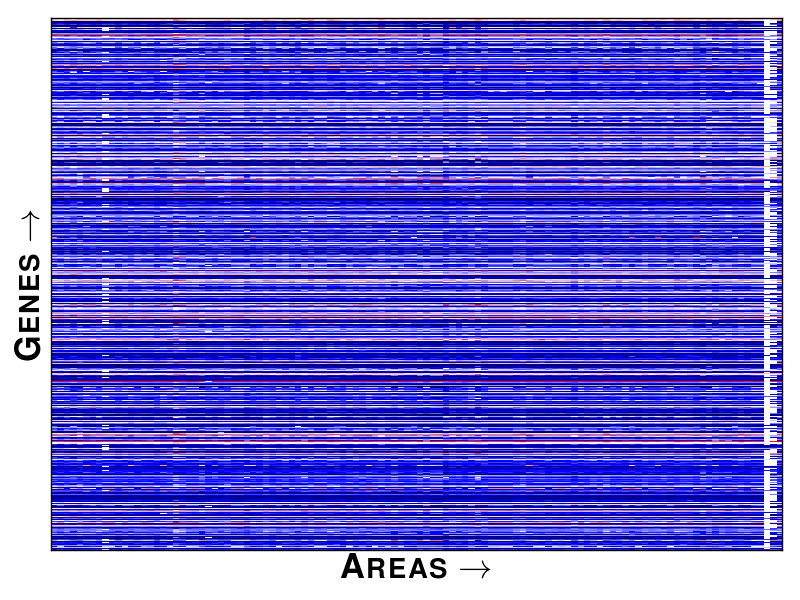
\includegraphics[scale=0.2]{expression-overall-for-methods.png}
			\end{minipage}
			
		};

		\node[above right of=gene-expression] (roi) 
		{
			\begin{minipage}{0.6\textwidth}
				\centering
				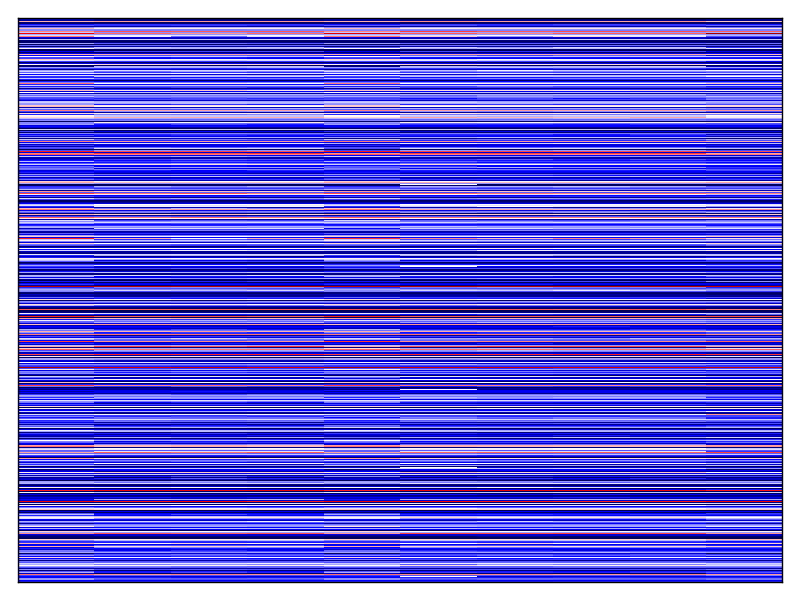
\includegraphics[scale=0.1]{expression-roi-for-methods.png}
			\end{minipage}
		};

		\node[below right of=gene-expression] (control)
{
			\begin{minipage}{0.25\textwidth}

				\centering
				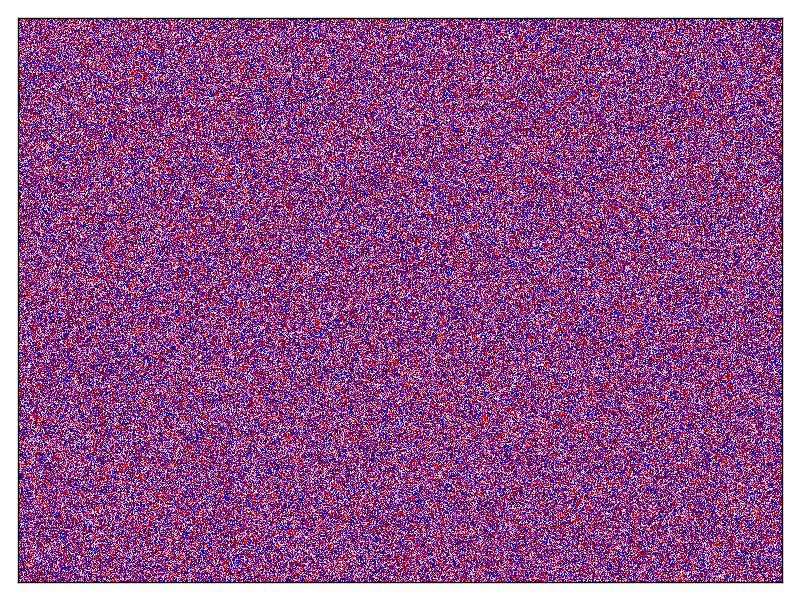
\includegraphics[scale=0.2]{expression-control-for-methods.png}
			\end{minipage}
		};

		\draw [arrow] (ABA) -- (gene-expression);
		\draw [arrow] (gene-expression) -- (roi);
		\draw [arrow] (gene-expression) -- (control);

		\draw [arrow,<->] (roi) -- node[above,rotate=90]{differential} node[above,rotate=-90] {expression} (control);
		
	\end{tikzpicture}
\vspace{-8em}
\begin{enumerate}
	\item[{.}] Dopaminergic signaling (GO:0007212)
	\item[{.}] Glutamatergic signaling (GO:0007215)
	\item[{.}] GABAergic signaling (GO:0007214)
	\item[{.}] Inflammation (GO:0006954)
	\item[{.}] Epigenetic regulation (GO:0040029)
\end{enumerate}

\end{document}